%------------------------------------------------------------------------
%Editar Diplomado
\hypertarget{cv:revisarCU}{\section{Revisar Caso de uso}} \label{sec:revisarCU}

	Esta funcionalidad le permitirá validar los casos de uso que fueron a enviados a revisión para que puedan ser liberados.
		\subsection{Procedimiento}

			%Pasos de procedimiento
			\begin{enumerate}
			
			\item Oprima el botón \IURevisar{} de algún registro existente de la pantalla \ref{fig:GestionarCU} ''Gestionar Casos de Uso''.
	
			\item Se mostrará la pantalla \ref{fig:RevisarCU} ''Revisar Caso de uso''.

			%Pantalla
			\begin{figure}[htbp!]
				\begin{center}
					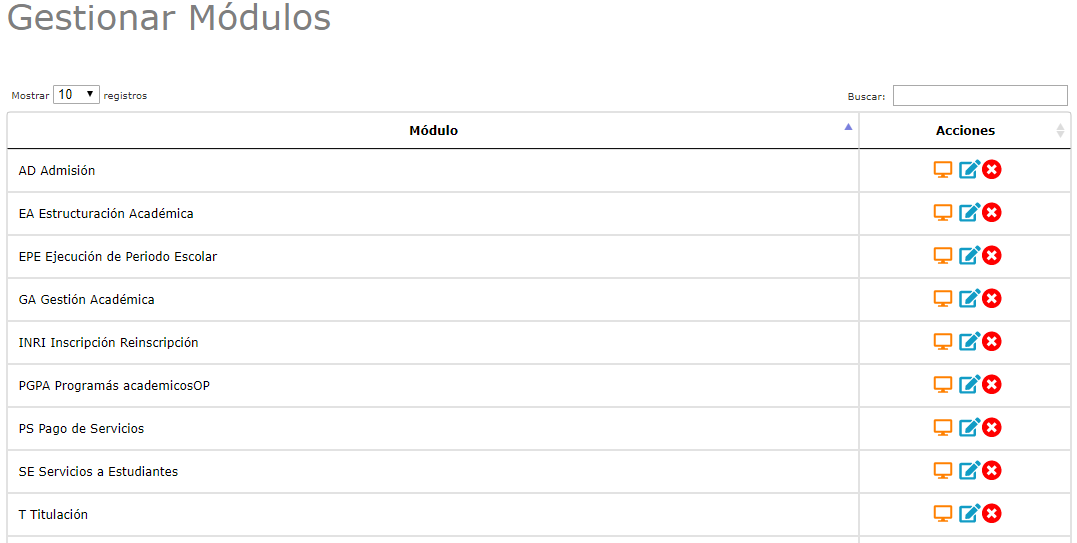
\includegraphics[scale=0.6]{roles/lider/casosUso/pantallas/IU5gestionarModulos}
					\caption{Revisar Caso de Uso}
					\label{fig:RevisarCU}
				\end{center}
			\end{figure}
		
				\item Marque la casilla dependiendo de si la información ingresada es correcta, en dado caso de que no sea asi ingrese las correcciones necesarias para que sean resultas de manera inmediata.
				
				\item Oprima el botón \IUAceptar.
				
				\item Se mostrará el mensaje \ref{fig:CURevisado} en la pantalla \ref{fig:GestionarCU} ''Gestionar Casos de Uso''.
				
				\begin{figure}[htbp!]
					\begin{center}
						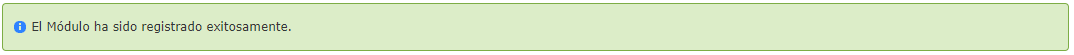
\includegraphics[scale=0.6]{roles/lider/casosUso/pantallas/IU5-1MSG1}
						\caption{MSG: Caso de Uso Revisado}
						\label{fig:CURevisado}
					\end{center}
				\end{figure}
			
			\end{enumerate}